\chapter{Hidrogen dan Blok s}\label{ch:b1:s-block}

Setiap ponsel, laptop, dan mobil listrik membawa baterai yang muatan
positifnya dibawa oleh ion litium. Litium itu sebagian besar berasal dari
dua tempat: tambang batuan keras di Australia dan dataran garam di
Pegunungan Andes, tempat air garam yang dipompa dari bawah kerak dibiarkan
menguap di bawah sinar matahari selama berbulan-bulan sampai garam-garam
litium dapat diendapkan darinya. Litium adalah \omterm{def:b1:s-block:families}{logam alkali} yang pertama,
golongan logam yang paling reaktif, dan tetangga-tetangganya --- natrium,
kalium, magnesium, dan kalsium --- memasok bahan kimia curah bagi
industri: soda kaustik, abu soda, kapur. Bab ini membuka kimia deskriptif
unsur-unsur dengan hidrogen dan \omterm{def:b1:periodicity:table}{blok} s, dengan memakai alat-alat dari
bab-bab sebelumnya --- energi ionisasi, \omterm{def:b1:nernst:electrode-potential}{potensial standar}, \omterm{def:b1:precipitation:solubility-product}{hasil kali
kelarutan} --- untuk menjelaskan perilaku unsur-unsur itu.

\begin{recall}
Energi ionisasi dan \omterm{def:b1:periodicity:electronegativity}{keelektronegatifan} (\cref{ch:b1:periodicity});
\omterm{def:b1:nernst:electrode-potential}{potensial standar} (\cref{ch:b1:nernst}); \omterm{def:b1:precipitation:solubility-product}{hasil kali kelarutan} dan
pengendapan hidroksida (\cref{ch:b1:precipitation}). Jilid sekolah
(kelas 10) telah mengelompokkan unsur-unsur ke dalam keluarga: \omterm{def:b1:s-block:families}{logam
alkali}, \omterm{def:b1:s-block:families}{logam alkali tanah}, halogen, gas mulia.
\end{recall}

\begin{omfigure}
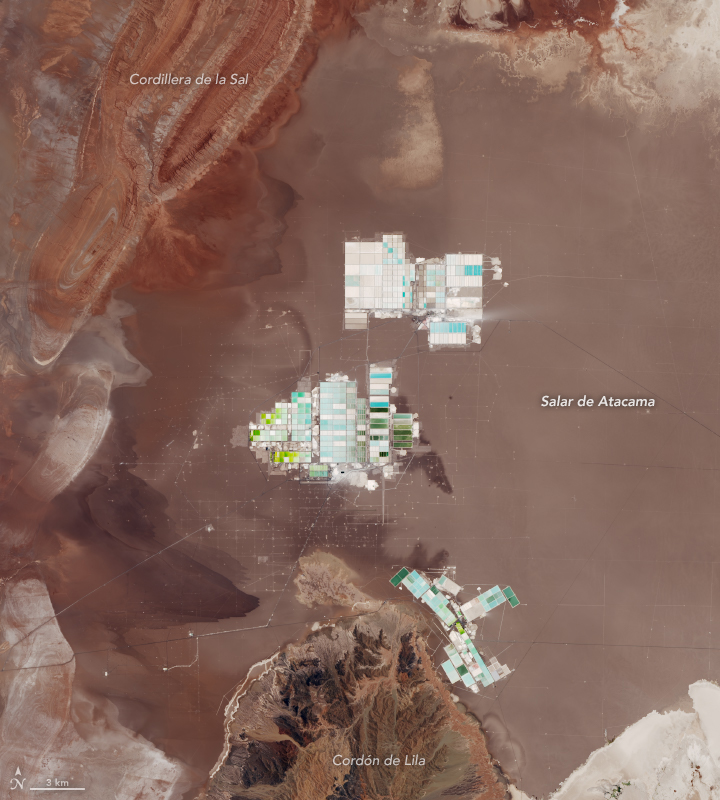
\includegraphics[width=0.48\linewidth]{images/book2/atacama-ponds.jpg}

{\small Kolam penguapan air garam litium di Salar de Atacama, dilihat dari
orbit (Landsat 8, 2018; NASA Earth Observatory, domain publik, Wikimedia
Commons). Warna setiap kolam berubah ketika air garam itu memekat dan
garam-garamnya mengkristal.}
\end{omfigure}

\section{Hidrogen dan hidrida}

Hidrogen mempunyai satu elektron: hidrogen dapat melepaskannya (\ce{H+},
yang dibawa air sebagai \ce{H3O+}), memakainya bersama (\omterm{def:b1:lewis-resonance-vsepr:lewis}{ikatan kovalen}),
atau menerima satu elektron (\ce{H-}, dengan \omterm{def:b1:quantum-numbers:configuration}{konfigurasi elektron} helium).
Mana yang terjadi bergantung pada pasangannya.

\begin{definition}[Hidrida]\label{def:b1:s-block:hydride}
\emph{Hidrida}\index{hidrida} adalah senyawa biner hidrogen dengan unsur
lain. \emph{Hidrida salin}\index{hidrida salin}, yang terbentuk dengan
\omterm{def:b1:s-block:families}{logam alkali} dan \omterm{def:b1:s-block:families}{logam alkali tanah} yang lebih berat (\ce{LiH}, \ce{NaH},
\ce{CaH2}), adalah padatan ionik yang mengandung \ce{H-}. \emph{Hidrida
kovalen}\index{hidrida kovalen}, yang terbentuk dengan unsur-unsur \omterm{def:b1:periodicity:table}{blok} p
(\ce{CH4}, \ce{NH3}, \ce{H2O}, \ce{HCl}), bersifat molekular.
\emph{Hidrida metalik}\index{hidrida metalik}, yang terbentuk dengan
beberapa logam transisi, adalah padatan yang hidrogennya menempati \omterm{def:b1:crystals-metals:site}{situs
interstisi} \omterm{def:b1:crystals-metals:lattice}{kisi} logam, sering dengan komposisi yang berubah-ubah.
\end{definition}

Ion \omterm{def:b1:s-block:hydride}{hidrida} adalah basa dan \omterm{def:b1:nernst:couple}{reduktor} yang sangat kuat: \omterm{def:b1:s-block:hydride}{hidrida salin}
bereaksi dengan air, \ce{NaH + H2O -> NaOH + H2}, dan dipakai sebagai zat
pengering untuk pelarut dan sebagai basa dalam sintesis organik
(\cref{ch:b1:alcohol-activation}). \omterm{def:b1:s-block:hydride}{Hidrida kovalen} \omterm{def:b1:periodicity:table}{periode} kedua
memperlihatkan kecenderungan \omterm{def:b1:periodicity:electronegativity}{keelektronegatifan} di sepanjang \omterm{def:b1:periodicity:table}{periode} itu:
\ce{CH4} tidak asam maupun basa, \ce{NH3} basa, \ce{H2O} amfoter, \ce{HF}
asam.

\section{Logam alkali}

\begin{definition}[Logam alkali dan logam alkali tanah]\label{def:b1:s-block:families}
\emph{Logam alkali}\index{logam alkali} (Li, Na, K, Rb, Cs, Fr) membentuk
\omterm{def:b1:periodicity:table}{golongan} 1, dengan satu \omterm{def:b1:quantum-numbers:configuration}{elektron valensi} \textit{ns}$^1$;
\emph{logam alkali tanah}\index{logam alkali tanah} (Be, Mg, Ca, Sr, Ba,
Ra) membentuk \omterm{def:b1:periodicity:table}{golongan} 2, dengan \textit{ns}$^2$. Unsur-unsur itu
membentuk \omterm{def:b1:periodicity:table}{blok} s.
\end{definition}

\begin{proposition}[Logam alkali adalah reduktor kuat]\label{prop:b1:s-block:reducing-power}
\omterm{def:b1:s-block:families}{Logam alkali} mempunyai \omterm{def:b1:periodicity:ionisation-energy}{energi ionisasi pertama} yang paling rendah dalam
\omterm{def:b1:periodicity:table}{periodenya} (Li \qty{5.39}{eV}, Na 5.14, K 4.34) dan \omterm{def:b1:nernst:electrode-potential}{potensial standar}
yang sangat negatif (\ce{Li+}/\ce{Li} $-3.04$~V, \ce{Na+}/\ce{Na} $-2.71$,
\ce{K+}/\ce{K} $-2.94$): logam-logam itu mereduksi air dan di alam hanya
ditemukan sebagai ion \ce{M+}.
\end{proposition}
% ledger: ie:Li, ie:Na, ie:K (E0 computed in figdata/bachelor-1/standard-potentials.py)

\begin{proof}
Satu elektron di luar teras gas mulia, jauh dari inti dan tertapis oleh
kulit-kulit dalam (\cref{ch:b1:periodicity}), mudah dilepaskan. Di dalam
air, ion \ce{M+} yang kecil terhidrasi kuat, sehingga potensial
pasangannya menjadi lebih rendah lagi. Dengan $E^\circ$ lebih dari
\qty{2.2}{V} di bawah garis air pada pH 7 ($-0.41$~V), reaksi
\ce{2M + 2H2O -> 2M+ + 2OH- + H2} mempunyai tetapan yang sangat besar
(\cref{prop:b1:nernst:equilibrium-constant}).
\end{proof}

\begin{omfigure}
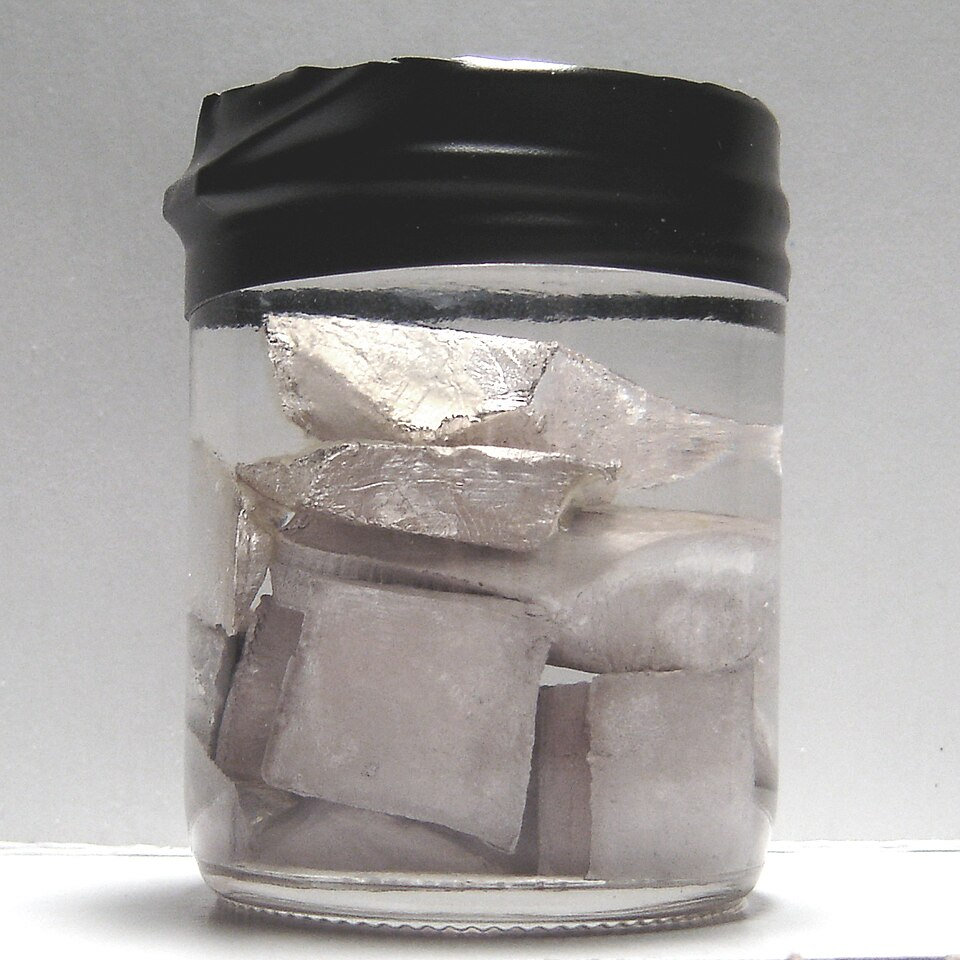
\includegraphics[height=4.6cm]{images/book2/sodium-oil.jpg}\hspace{0.8em}%
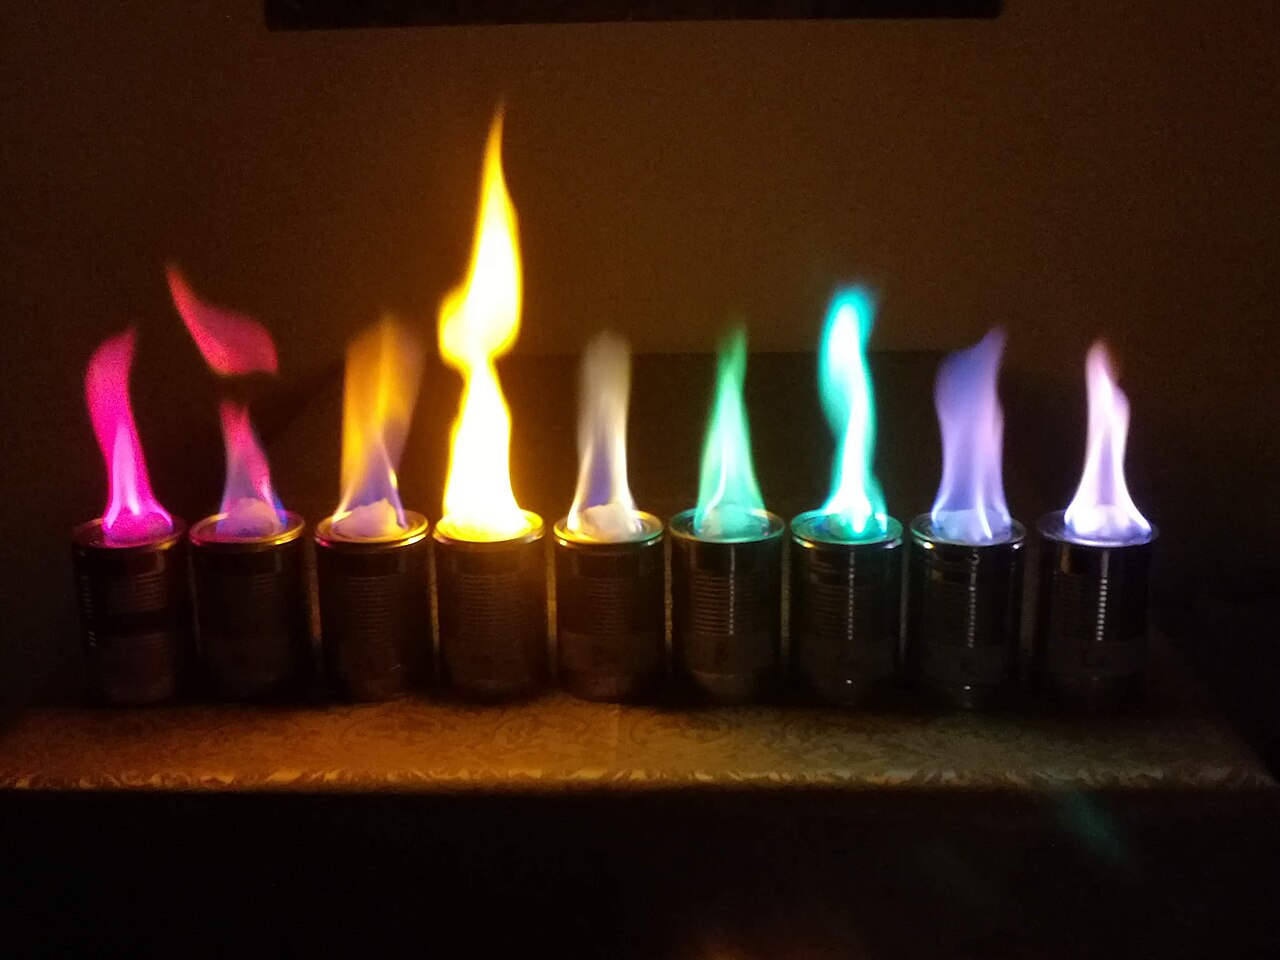
\includegraphics[height=4.6cm]{images/book2/flame-colours.jpg}

{\small Kiri: natrium disimpan di bawah minyak mineral, jauh dari udara
dan kelembapan (foto Justin Urgitis, CC BY-SA 2.5). Kanan: warna nyala,
dari kiri ke kanan, senyawa litium, stronsium, kalsium, natrium, barium,
boron, tembaga, sesium, dan kalium: elektron yang tereksitasi dalam nyala
kembali ke tingkat yang lebih rendah sambil memancarkan cahaya pada
panjang gelombang yang khas untuk setiap unsur
(\cref{ch:b1:quantum-numbers}) (foto Hegelrast, CC BY-SA 4.0). Keduanya
dari Wikimedia Commons.}
\end{omfigure}

\begin{inthelab}[Sebuah demonstrasi, bukan percobaan]
Reaksi natrium dengan air hanya diperagakan oleh guru, di balik layar
pengaman, dengan sepotong logam sebesar biji lentil yang dijatuhkan ke
dalam bak besar berisi air yang mengandung fenolftalein: logam itu
meleleh menjadi bola yang meluncur, hidrogen berdesis, dan jejak merah
muda memperlihatkan hidroksida yang terbentuk. Kalium menyalakan
hidrogennya. Potongan yang lebih besar meledak. Natrium dipotong di bawah
minyak, dipegang dengan penjepit, dan sisanya dirusak dengan etanol,
tidak pernah dengan air.
\end{inthelab}

Litium adalah pengecualian dalam \omterm{def:b1:periodicity:table}{golongannya}: ionnya paling kecil, paling
kuat terhidrasi, sehingga potensialnya paling negatif, tetapi paling
lambat bereaksi dengan air. Senyawa-senyawanya menyerupai senyawa
magnesium (litium karbonat dan litium fosfat sukar larut, seperti halnya
senyawa magnesium), sebuah hubungan diagonal dalam tabel periodik. \omterm{def:b1:s-block:families}{Logam
alkali} diproduksi melalui elektrolisis leburan kloridanya, karena tidak
ada \omterm{def:b1:nernst:couple}{reduktor} kimia yang cukup kuat; reaksi elektrode dalam sel semacam
itu dipelajari dalam jilid Tahun~2.

\section{Senyawa natrium dalam industri}

\begin{definition}[Sifat oksida]\label{def:b1:s-block:oxide-character}
\emph{Oksida basa}\index{oksida basa} bereaksi dengan air menghasilkan
hidroksida, atau dengan asam menghasilkan garam (\ce{Na2O}, \ce{CaO});
\emph{oksida asam}\index{oksida asam} bereaksi dengan air menghasilkan
asam, atau dengan basa menghasilkan garam (\ce{CO2}, \ce{SO3},
\ce{P4O10}); \emph{oksida amfoter}\index{oksida amfoter} bereaksi dengan
asam maupun basa (\ce{Al2O3}, \ce{ZnO}). Di sepanjang \omterm{def:b1:periodicity:table}{periode}, oksida
berubah dari basa (logam, kiri) menjadi asam (nonlogam, kanan).
\end{definition}

Natrium hidroksida dibuat melalui elektrolisis air garam (proses
klor-alkali, yang juga menghasilkan klorin dan hidrogen). Natrium
karbonat, abu soda, yang dipakai untuk kaca, detergen, dan ekstraksi
litium, ditambang sebagai mineral trona atau dibuat dari garam dan batu
kapur: pada tahun 2025 dunia memproduksi sekitar 71 juta ton, 19 juta dari
endapan alam dan 52 juta secara sintetis, sebagian besar melalui proses
Solvay.
% ledger: usgs:sodaash-total-2025, usgs:sodaash-natural-2025, usgs:sodaash-synthetic-2025

\begin{proposition}[Proses Solvay]\label{prop:b1:s-block:solvay}
Proses Solvay mengubah natrium klorida dan kalsium karbonat menjadi
natrium karbonat dan kalsium klorida, \ce{2NaCl + CaCO3 -> Na2CO3 +
CaCl2}, melalui tahap-tahap yang mendaur ulang amonia dan karbon
dioksida.
\end{proposition}

\begin{proof}
Tahap-tahapnya: (1) \ce{CaCO3 -> CaO + CO2} (tanur); (2) \ce{NaCl + NH3 +
CO2 + H2O -> NaHCO3 + NH4Cl} (karbonasi air garam beramonia;
hidrogenkarbonat, garam yang paling sukar larut di antara yang ada,
mengendap); (3)
\ce{2NaHCO3 -> Na2CO3 + CO2 + H2O} (kalsinasi); (4) \ce{CaO + H2O ->
Ca(OH)2}; (5) \ce{Ca(OH)2 + 2NH4Cl -> CaCl2 + 2NH3 + 2H2O} (pemulihan
amonia). Dengan menjumlahkan $(1) + 2\times(2) + (3) + (4) + (5)$, \ce{NH3},
\ce{CO2}, \ce{NH4Cl}, \ce{NaHCO3}, \ce{CaO}, \ce{Ca(OH)2}, dan air saling
meniadakan: \ce{2NaCl + CaCO3 -> Na2CO3 + CaCl2}.
\end{proof}

\begin{omfigure}
\begin{tikzpicture}[font=\small, >={Stealth}, box/.style={draw, rounded corners, fill=omDef!8, minimum width=2.6cm, minimum height=0.8cm, align=center}]
  \node[box] (kiln) at (0,0) {tanur kapur\\\ce{CaCO3 -> CaO + CO2}};
  \node[box] (tower) at (5.3,0) {menara karbonasi\\\ce{NaHCO3} mengendap};
  \node[box] (calc) at (10.2,0) {kalsinator\\\ce{NaHCO3} $\to$ \ce{Na2CO3}};
  \node[box] (slake) at (0,-2.6) {pemadaman kapur\\\ce{CaO + H2O -> Ca(OH)2}};
  \node[box] (still) at (5.3,-2.6) {penyuling amonia\\\ce{NH4Cl + Ca(OH)2}};
  \draw[->, thick] (kiln) -- node[above] {\ce{CO2}} (tower);
  \draw[->, thick] (tower) -- node[above, font=\scriptsize] {\ce{NaHCO3}} (calc);
  \draw[->, thick] (calc.north) -- ++(0,0.6) -| node[pos=0.25, above] {\ce{CO2} didaur ulang} (tower.north);
  \draw[->, thick] (kiln) -- node[left] {\ce{CaO}} (slake);
  \draw[->, thick] (slake) -- node[above, font=\scriptsize] {\ce{Ca(OH)2}} (still);
  \draw[->, thick] (tower) -- node[right] {\ce{NH4Cl}} (still);
  \draw[->, thick] (still.east) -- ++(1.2,0) |- node[pos=0.25, right] {\ce{NH3} didaur ulang} ($(tower.east)+(0,-0.25)$);
  \draw[<-, thick] (tower.north west) -- ++(-0.5,0.6) node[above] {air garam \ce{NaCl}};
  \draw[->, thick] (calc.east) -- ++(0.8,0) node[right] {\ce{Na2CO3}};
  \draw[->, thick] (still.south) -- ++(0,-0.6) node[below] {\ce{CaCl2}};
\end{tikzpicture}

{\small Proses Solvay. Karbon dioksida dan amonia beredar dalam
lingkaran; garam dan batu kapur masuk, abu soda dan kalsium klorida
keluar.}
\end{omfigure}

\begin{omfigure}
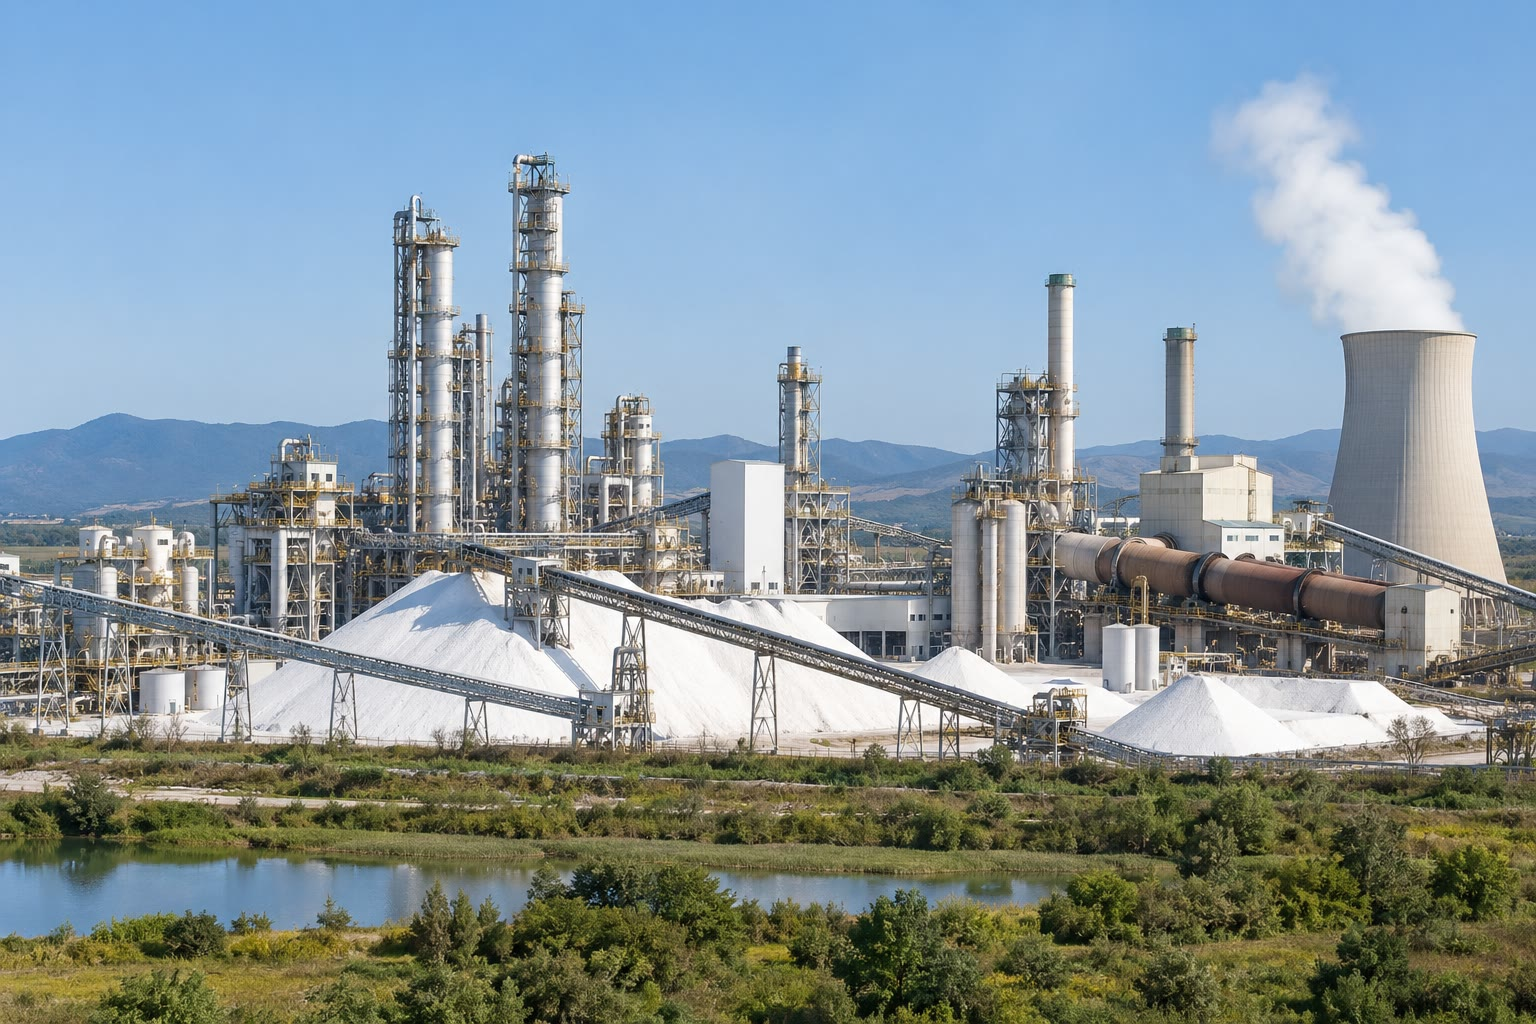
\includegraphics[width=0.55\linewidth]{images/book2/ai/b1-26-soda-ash-plant.jpg}

{\small Pabrik abu soda: tanur kapur, menara karbonasi, dan timbunan
natrium karbonat.}
\end{omfigure}

\begin{method}[Neraca massa pada diagram alir]\label{met:b1:s-block:mass-balance}
\begin{enumerate}
  \item Tuliskan persamaan keseluruhannya (jumlah tahap-tahapnya, dengan
        spesi yang didaur ulang saling meniadakan).
  \item Dari produk yang diinginkan, hitunglah jumlah bahan baku dengan
        persamaan keseluruhan itu, lalu koreksilah untuk \omterm{def:b1:extent-q-and-k:fractional-extent}{rendemen} setiap
        tahap.
  \item Untuk spesi yang didaur ulang, hitunglah hanya tambahan yang
        diperlukan untuk menggantikan kehilangannya.
  \item Periksalah neraca setiap unsur antara masukan dan keluaran.
\end{enumerate}
\end{method}

\section{Logam alkali tanah}

Magnesium dan kalsium kurang reaktif daripada \omterm{def:b1:s-block:families}{logam alkali} (energi
ionisasinya lebih tinggi: Mg \qty{7.65}{eV}, Ca 6.11; ada dua elektron
yang harus dilepaskan), tetapi tetap merupakan \omterm{def:b1:nernst:couple}{reduktor} kuat ($E^\circ$
\ce{Mg^2+}/\ce{Mg} $-2.36$~V). Magnesium terbakar di udara dengan cahaya
putih yang menyilaukan; lapisan oksidanya melindunginya pada suhu kamar.
Magnesium diperoleh dari air laut dengan mengendapkan hidroksidanya
memakai kapur, $\mathrm{p}K_s = 11.25$ (\cref{ch:b1:precipitation}).
% ledger: ie:Mg, ie:Ca

\begin{proposition}[Siklus kapur]\label{prop:b1:s-block:lime-cycle}
Batu kapur, kapur tohor, kapur padam, dan batu kapur lagi membentuk
sebuah siklus: \ce{CaCO3 -> CaO + CO2} (dipanaskan dalam tanur);
\ce{CaO + H2O -> Ca(OH)2} (pemadaman, sangat eksoterm);
\ce{Ca(OH)2 + CO2 -> CaCO3 + H2O} (pengerasan adukan kapur di udara).
Siklus itu secara keseluruhan tidak mengubah apa pun secara kimia,
tetapi menyimpan dan melepaskan energi dan karbon dioksida.
\end{proposition}

\begin{proof}
Jika ketiga persamaan dijumlahkan, setiap spesi saling meniadakan.
Penguraian karbonat memerlukan kalor, yang dilepaskan kembali pada kedua
tahap lainnya; \ce{CO2} yang dilepaskan di dalam tanur diserap kembali,
secara perlahan, oleh adukan itu.
\end{proof}

\begin{omfigure}
\begin{tikzpicture}[font=\small, >={Stealth}]
  \node[draw, rounded corners, fill=omDef!8] (a) at (90:2.0) {\ce{CaCO3} batu kapur};
  \node[draw, rounded corners, fill=omDef!8, align=center] (b) at (-30:2.0) {\ce{CaO}\\kapur tohor};
  \node[draw, rounded corners, fill=omDef!8, align=center] (c) at (210:2.0) {\ce{Ca(OH)2}\\kapur padam};
  \draw[->, thick] (a) to[bend left=25] node[right, align=left] {kalor\\$-\ce{CO2}$} (b);
  \draw[->, thick] (b) to[bend left=25] node[below] {$+\ce{H2O}$} (c);
  \draw[->, thick] (c) to[bend left=25] node[left, align=right] {$+\ce{CO2}$\\$-\ce{H2O}$} (a);
\end{tikzpicture}

{\small Siklus kapur, dari batu kapur ke adukan dan kembali ke kalsium
karbonat.}
\end{omfigure}

\section{Litium}

\begin{omfigure}
\begin{tikzpicture}
\begin{axis}[
  xbar, width=0.78\linewidth, height=5.4cm, xmin=0, xmax=110,
  symbolic y coords={CA,ML,BR,AR,ZW,CL,CN,AU}, ytick=data,
  yticklabels={Kanada, Mali, Brasil, Argentina, Zimbabwe, Chili, Tiongkok, Australia},
  xlabel={litium yang ditambang pada 2025 (ribu ton Li, perkiraan)}, bar width=8pt,
  nodes near coords, every node near coord/.append style={font=\scriptsize},
  tick label style={font=\small}, label style={font=\small}, enlarge y limits=0.1]
\addplot[fill=omDef!45, draw=omDef] coordinates {(5.6,CA) (9.4,ML) (12,BR) (23,AR) (28,ZW) (56,CL) (62,CN) (92,AU)};
\end{axis}
\end{tikzpicture}

{\small Produsen litium terbesar pada tahun 2025 (perkiraan; total dunia
sekitar \num{290000} ton litium). Australia menambang batuan keras
(spodumen); Chili dan Argentina memompa air garam.}
% ledger: usgs:li-canada-2025, usgs:li-mali-2025, usgs:li-brazil-2025, usgs:li-argentina-2025, usgs:li-zimbabwe-2025, usgs:li-chile-2025, usgs:li-china-2025, usgs:li-australia-2025, usgs:li-world-2025
\end{omfigure}

Air garam dipekatkan melalui penguapan, magnesium dihilangkan dengan
kapur, dan litium karbonat diendapkan dengan abu soda. Litium karbonat
mempunyai sifat yang tidak biasa, yaitu lebih sukar larut dalam keadaan
panas daripada dingin: \qty{1.31}{\percent} massa pada
\qty{20}{\celsius}, \qty{0.84}{\percent} pada \qty{80}{\celsius},
\qty{0.71}{\percent} pada \qty{100}{\celsius}. Karena itu, zat itu
diendapkan dari larutan panas, seperti yang dihitung dalam soal akhir
pekan.
% ledger: sol:Li2CO3-20, sol:Li2CO3-80, sol:Li2CO3-100

\section{Latihan}

\begin{exercise}[$\star$]\label{exo:b1:s-block:1}
Golongkan sebagai \omterm{def:b1:s-block:hydride}{hidrida salin}, kovalen, atau metalik: \ce{KH}, \ce{SiH4},
\ce{CaH2}, \ce{H2S}, \ce{PdH_{0.6}}. Tuliskan reaksi \ce{CaH2} dengan air.
\end{exercise}

\begin{exercise}[$\star$]\label{exo:b1:s-block:2}
Tuliskan reaksi litium, natrium, dan kalium dengan air, serta reaksi
magnesium dengan asam klorida encer.
\end{exercise}

\begin{exercise}[$\star$]\label{exo:b1:s-block:3}
Golongkan sebagai \omterm{def:b1:s-block:oxide-character}{oksida basa}, asam, atau amfoter: \ce{Na2O}, \ce{MgO}, \ce{Al2O3},
\ce{SiO2}, \ce{SO3}, \ce{ZnO}, \ce{CO2}. Tuliskan satu reaksi untuk setiap jenis.
\end{exercise}

\begin{exercise}[$\star$]\label{exo:b1:s-block:4}
Hitunglah tetapan reaksi \ce{2Na + 2H2O -> 2Na+ + 2OH- + H2} pada pH 14
dari \omterm{def:b1:nernst:electrode-potential}{potensial standarnya}.
\end{exercise}

\begin{exercise}[$\star\star$]\label{exo:b1:s-block:5}
Jelaskan warna nyala litium (merah) dan natrium (kuning) dengan memakai
\omterm{def:b1:quantum-numbers:energy-level}{tingkat energi} atom (\cref{ch:b1:quantum-numbers}). Berapakah energi
sebuah foton kuning pada \qty{589}{nm}?
\end{exercise}

\begin{exercise}[$\star\star$]\label{exo:b1:s-block:6}
Hitunglah massa batu kapur (\ce{CaCO3} murni) dan natrium klorida yang
diperlukan untuk satu ton abu soda melalui proses Solvay, dengan \omterm{def:b1:extent-q-and-k:fractional-extent}{rendemen}
keseluruhan \qty{90}{\percent} terhadap natrium klorida.
\end{exercise}

\begin{exercise}[$\star\star$]\label{exo:b1:s-block:7}
Air laut mengandung sekitar \qty{1.3}{g/L} magnesium (data latihan). Pada
pH berapa magnesium hidroksida mulai mengendap? Berapa massa kapur padam
yang mengendapkan magnesium dalam \qty{1.0}{m^3}?
\end{exercise}

\begin{exercise}[$\star\star$]\label{exo:b1:s-block:8}
Mengapa litium bereaksi lebih lambat dengan air daripada kalium, padahal
\omterm{def:b1:nernst:electrode-potential}{potensial standarnya} lebih rendah? Bedakan termodinamika dan kinetika.
\end{exercise}

\begin{exercise}[$\star\star$]\label{exo:b1:s-block:9}
Hitunglah massa kapur tohor yang diperoleh dari satu ton batu kapur dan
volume \ce{CO2} yang dilepaskan, pada \qty{25}{\celsius} dan \qty{1}{bar}.
\end{exercise}

\begin{exercise}[$\star\star\star$]\label{exo:b1:s-block:10}
Dunia menambang sekitar \num{290000} ton litium pada tahun 2025. Berapa
massa litium karbonat yang setara dengan jumlah itu? Jika sebuah baterai
mobil berisi \qty{8}{kg} litium (data latihan), berapa baterai yang dapat
dipasoknya?
\end{exercise}

\begin{exercise}[$\star\star\star$]\label{exo:b1:s-block:11}
Tunjukkan dari data dalam bab ini bahwa \omterm{def:b1:precipitation:solubility}{kelarutan} litium karbonat turun
ketika suhu naik, dan jelaskan mengapa pengendapannya dalam keadaan panas
meningkatkan perolehan dari air garam.
\end{exercise}

\begin{exercise}[$\star\star\star$]\label{exo:b1:s-block:12}
Pada tahap (2) proses Solvay, larutan mengandung \ce{Na+}, \ce{NH4+},
\ce{Cl-}, dan \ce{HCO3-}. Jelaskan mengapa natrium hidrogenkarbonat yang
mengendap dan bukan amonium klorida, dan mengapa proses itu memerlukan
amonia dan bukan natrium hidroksida.
\end{exercise}

\section{Soal: Litium dari Air Garam}

\begin{problem}[{Soal akhir pekan --- memekatkan air garam litium,
menghilangkan magnesium dengan kapur, mengendapkan litium karbonat dengan
abu soda, dan massa litium karbonat yang diperoleh dari satu meter kubik}]
\label{pb:b1:s-block:1}
Air garam yang dipompa dari bawah sebuah dataran garam mengandung
\qty{1.5}{g/L} litium dan \qty{0.60}{g/L} magnesium (sebagai ion, dengan
banyak natrium klorida). Penguapan di dalam kolam memekatkannya empat
kali. Satu meter kubik air garam pekat itu lalu diolah: kapur
menghilangkan magnesium, abu soda menghilangkan kalsium, dan akhirnya abu
soda panas mengendapkan litium karbonat pada \qty{80}{\celsius}. Data:
massa molar (\unit{g/mol}) Li 6.9, Mg 24.3, \ce{Ca(OH)2} 74.1,
\ce{Na2CO3} 106.0, \ce{Li2CO3} 73.8; $\mathrm{p}K_s$ \ce{Mg(OH)2} 11.25,
\ce{CaCO3} 8.30; $\mathrm{p}K_e = 14.00$; \omterm{def:b1:precipitation:solubility}{kelarutan} \ce{Li2CO3}
\qty{0.84}{\percent} massa pada \qty{80}{\celsius}; anggaplah cairan
akhirnya \qty{1.00}{m^3} dengan massa jenis \qty{1.0}{kg/L}.

\medskip
\noindent\textbf{Bagian I --- Pemekatan.}
\begin{enumerate}
  \item Hitunglah konsentrasi litium dan magnesium dalam air garam pekat.
  \item Berapa volume air yang menguap per meter kubik air garam pekat?
  \item Mengapa dipakai penguapan oleh matahari dan bukan pemanasan?
  \item Garam manakah yang paling dahulu mengkristal di dalam kolam, dan
        mengapa?
  \item Hitunglah jumlah litium dan magnesium dalam satu meter kubik.
  \item Mengapa magnesium harus dihilangkan sebelum litium diendapkan?
\end{enumerate}

\medskip
\noindent\textbf{Bagian II --- Menghilangkan magnesium dan kalsium.}
\begin{enumerate}[resume]
  \item Tuliskan reaksi ion magnesium dengan kapur padam.
  \item Hitunglah massa kapur padam yang diperlukan (stoikiometris).
  \item Pada pH berapa \qty{99.9}{\percent} magnesium telah mengendap?
  \item Mengapa litium tidak mengendap sebagai hidroksidanya?
  \item Tuliskan penghilangan kalsium yang dimasukkan, dengan abu soda.
  \item Hitunglah massa abu soda yang diperlukan untuk tahap itu.
\end{enumerate}

\medskip
\noindent\textbf{Bagian III --- Litium karbonat.}
\begin{enumerate}[resume]
  \item Tuliskan pengendapan litium karbonat.
  \item Hitunglah massa abu soda yang diperlukan untuk litium.
  \item Hitunglah massa teoretis litium karbonat.
  \item Mengapa pengendapan dilakukan pada \qty{80}{\celsius}?
  \item Berapa massa litium karbonat yang tetap terlarut dalam cairan itu?
  \item Bagaimana endapan itu dicuci tanpa kehilangan banyak darinya?
\end{enumerate}

\medskip
\noindent\textbf{Bagian IV --- Neraca.}
\begin{enumerate}[resume]
  \item Hitunglah massa litium karbonat yang diperoleh kembali.
  \item Hitunglah perolehan litium.
  \item Usulkan apa yang dilakukan terhadap cairan itu.
  \item Bandingkan litium dalam satu meter kubik dengan produksi dunia
        tahun 2025: berapa meter kubik yang setara dengan produksi itu?
  \item Nyatakan massa litium karbonat yang diperoleh kembali per meter
        kubik air garam pekat.
\end{enumerate}
\end{problem}
